\documentclass[a4paper,12pt]{article}
\usepackage[utf8]{inputenc}
\usepackage{amsmath}
\usepackage{amssymb}
\usepackage{hyperref}
\usepackage{listings}
\usepackage{xcolor}
\usepackage{fancyhdr}
\usepackage{geometry}
\usepackage{graphicx}
\usepackage{verbatim}

\geometry{margin=1in}

% Define Python style for listings
\lstset{
    language=Python,
    basicstyle=\ttfamily\small,
    keywordstyle=\color{blue},
    commentstyle=\color{gray},
    stringstyle=\color{green},
    numbers=left,
    numberstyle=\tiny,
    stepnumber=1,
    numbersep=8pt,
    showstringspaces=false,
    breaklines=true,
    frame=single,
}

\begin{document}

\title{\textbf{NLP Assignment 01 Report}}
\author{Hammad Sajid (hs07606)}
\date{13/09/2024}

\maketitle

\tableofcontents
\newpage

\section{Task 01: Resolving Ambiguities Between Date Formats}

\subsection{Algorithm}

The Python script I implemented resolves ambiguities between two date formats: \texttt{DD/MM/YYYY} and \texttt{MM/DD/YYYY}. Here's the method used to resolve the format:

\begin{itemize}
    \item \textbf{Extract Dates Using Regular Expressions:} The script uses a regular expression \verb|\b(0?[1-9]|[12][0-9]|3[01])/(0?[1-9]|1[0-2])/([12][0-9]{3})\b| to extract dates that could either be in \texttt{DD/MM/YYYY} or \texttt{MM/DD/YYYY} format. This pattern matches any day (1-31), month (1-12), and a four-digit year (starting with 19 or 20).
    
    \item \textbf{Determining the Date Format:}
    \begin{itemize}
        \item \textbf{Logical Assumptions:} If the day exceeds 12, the format is assumed to be \texttt{DD/MM/YYYY} because months can only go up to 12. If the months exceed 12, the format is assumed to be \texttt{MM/DD/YYYY}.
        
        \item \textbf{Contextual Clues (for test cases):} The script checks for specific phrases such as \emph{"held on"}, \emph{"registration deadline"}, \emph{"scheduled for"}, and \emph{"due on"} required for test cases. If such phrases are found, the script assumes the format is \texttt{DD/MM/YYYY} since  
        
        \item \textbf{Month Names:} The script looks for month names in the context surrounding the date to identify potential months in word form, which can help confirm the date format. 
        
        \item \textbf{British and American English:} While detecting British and American English words helped in some cases, it was not always reliable. For example, a text written in American English might contain \texttt{DD/MM/YYYY} dates if it’s written by someone from a different region, making it less reliable to base decisions on language clues alone.
    \end{itemize}
\end{itemize}

% \subsection{Code}

% \begin{lstlisting}
%     import re

% def read_file(file_path):
%     """Reads the input file and returns its content as a string."""
%     with open(file_path, 'r') as file:
%         lines = file.readlines()
%     return lines

% def extract_dates(text):

%     #regular expression (referenced from internet)
%     datepattern = r'\b(0?[1-9]|[12][0-9]|3[01])/(0?[1-9]|1[0-2])/([12][0-9]{3})\b'

%     matchingdates = re.finditer(datepattern, text)

%     # for match in matchingdates:
%     #     print(match.group(0))
    
%     datesformat = []

%     for match in matchingdates:
%         datestring = match.group()
%         day, month, year = match.groups()
%         day, month, year = int(day), int(month), int(year)

%         # print("the datestring is: ", datestring)
%         # print("the day is: ", day)
%         # print("the month is: ", month)
%         # print("the year is: ", year)
%         # print(text)

%         typeofformat = determine_format(day, month, text)
%         datesformat.append((datestring, typeofformat, text))

%     return datesformat

% def determine_format(day, month, context):

%     #checking mention of any month for generalised test cases.
%     contextualwords = ["held on", "registration deadline", "scheduled for", "due on"]
%     month_names = ["january", "february", "march", "april", "may", "june", "july", "august", "september", "october", "november", "december"]
%     british_words = ['colour', 'flavour', 'labour', 'neighbour', 'rumour']
%     american_words = ['color', 'flavor', 'labor', 'neighbor', 'rumor']

%     #basic test cases for direct checking.
%     if day > 12:
%         return 'DD/MM/YYYY'
%     elif month > 12:
%         return 'MM/DD/YYYY'
%     else:
%         context = context.lower()
        
%         #contextual words based on test cases
%         if any(contextualwords in context for contextualwords in contextualwords):
%             if day <= 12 and month <= 12:
%                 return 'DD/MM/YYYY'
            
%         #check for > 1 mention of months to pass the test case
%         if any(month_name in context for month_name in month_names):
%             # Check for multiple months in the context for test case
%             if sum(month_name in context for month_name in month_names) > 1:
%                 return 'Ambiguous'
            
%             if day <= 12 and month <= 12:
%                 return 'MM/DD/YYYY'

%         if any(word in context for word in british_words):
%             # Assume UK format (DD/MM/YYYY) if British English words are found
%             return "DD/MM/YYYY"
%         if any(word in context for word in american_words):
%             # Assume US format (MM/DD/YYYY) if American English words are found
%             return "MM/DD/YYYY"

%         return 'Ambiguous'


% def write_output(dates_with_format, output_file):
%     with open(output_file, 'a') as file:
%         for date, format_type, context in dates_with_format:
%             file.write(f"{date} - {format_type} - Context: {context}\n")

% def main():
%     # input
%     input_file_path = 'date_format_dd_mm_yyyy.txt'
%     # output
%     output_file_path = 'HammadSajid_hs07606.txt'

%     # Read input
%     lines = read_file(input_file_path)

%     for line in lines:
%         # Extract dates with surrounding context and determine their formats
%         dates_with_format = extract_dates(line.strip())

%         write_output(dates_with_format, output_file_path)

%     return

% if __name__ == "__main__":
%     main()
% \end{lstlisting}

\subsection{Output}

%add picture here

\begin{figure}[h!]
    \centering
    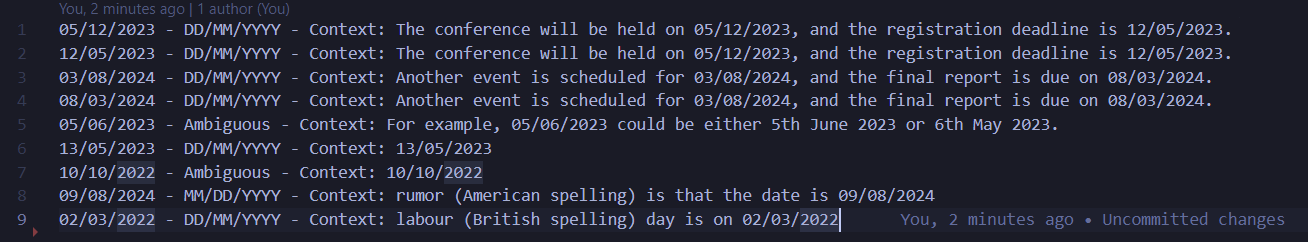
\includegraphics[width=\textwidth]{Fig1.png}
    \caption{Output of task 01.}
    \label{fig:output_image}
\end{figure}


The first and second output is DD/MM/YYYY as it should be since based on my assumption 
the conference will be held after the registration deadline. For the third and fourth 
output, the event should be held after the final report. For the fifth, it should be 
ambiguous as mentioned in the test case already.

I added 4 more test cases for my checking of code:

\begin{itemize}
    \item 13/05/2023 should be DD/MM/YYYY since MM could not be greater than 12.
    \item 10/10/2022 should be ambiguous because of no context.
    \item 09/08/2024 should be MM/DD/YYYY because of rumor spelling that makes it American English.
    \item 02/03/2022 should be DD/MM/YYYY  because of labour spelling that makes it British English.
\end{itemize}

\subsection{Challenges and Difficulties}

This was a very ambiguous question with infinite possibilities which, in my opinion, cannot be done completely using Python coding alone but would require a model to be trained to identify the format with higher accuracy. However, I tried to consider as many cases as possible and generalize my code. Implementing the code was easy, but handling the immense variety of cases and arranging the conditions carefully was crucial.

The code can be found in the file \textbf{date\_format$.$py} and the output can be found in \textbf{HammadSajid\_hs07606$.$txt} file.

\section{Task 02: First 10 Merged Pairs in WordPiece Algorithm}

\subsection{First 10 Pairs}

The first 10 pairs merged by my algorithm are presented below:

\begin{verbatim}
    First 10 pairs merged by the algorithm with their frequency scores:
    Pair: ('1', '##0'), Score: 1.000000
    Pair: ('o', '##f'), Score: 0.250000
    Pair: ('##f', '##y'), Score: 0.500000
    Pair: ('e', '##x'), Score: 0.250000
    Pair: ('##m', '##p'), Score: 0.166667
    Pair: ('##q', '##u'), Score: 0.142857
    Pair: ('##b', '##u'), Score: 0.166667
    Pair: ('##mp', '##l'), Score: 0.083333
    Pair: ('##bu', '##l'), Score: 0.090909
    Pair: ('ex', '##a'), Score: 0.071429
\end{verbatim}

I verified the first few manually to ensure correctness, but not all of them since the text was too long, and calculating it manually would be too time-consuming.

\subsection{Challenges and Difficulties}

There were no significant challenges in this task. The main challenge was identifying which data structure to use for tracking pairs' counts. A dictionary was most suitable for its ability to manipulate key-value pairs. Ensuring correct list indexing was another minor issue, but printing debug information during development helped ensure the code worked as intended. Other than that, I faced some problems in assigning \#\# before characters during tokenization.
Initially, I did not add any \#\# in my code which was giving a very different output, but when I ran the HuggingFace's implementation seperately on Google Collab and ran the test script on their code, I realized that I had to add \#\# for correct outputs. Luckily as soon as I added \#\# prefix, my code started working as desired.

I implemented the WordPiece algorithm as explained in this video:

\href{https://youtu.be/qpv6ms_t_1A?si=F-v5NCcJ6SvIVLvX}{HuggingFace Video on WordPiece Algorithm}.

I also referenced the WordPiece algorithm presented here:

\href{https://huggingface.co/learn/nlp-course/en/chapter6/6}{HuggingFace Course - WordPiece Algorithm}.

\section{Task 03: Urdu Text Tokenization}

\subsection{Using Regular Expressions}

\begin{lstlisting}
    import re


    def read_urdu_text(file_path):
        with open(file_path, 'r', encoding='utf-8') as file:
            text = file.read()
        return text
    
    
    
    def tokenize_urdu_text(text):
        # Regular expression pattern for Urdu words
        urdu_word_pattern = r'\b[\u0600-\u06FF]+\b'
    
        tokens = re.findall(urdu_word_pattern, text)
        return tokens
    
    
    def write_tokens_to_file(tokens, output_file_path):
        with open(output_file_path, 'w', encoding='utf-8') as file:
            for token in tokens:
                file.write(token + '\n')
    
    
    if __name__ == "__main__":
    
        # Define file paths
        input_file_path = "urdu_text_input.txt"
        output_file_path = "urdu_tokens_output_re.txt"
    
        urdu_text = read_urdu_text(input_file_path)
    
        tokens = tokenize_urdu_text(urdu_text)
    
        write_tokens_to_file(tokens, output_file_path)
    
        print("Tokenization complete. Tokens have been written to", output_file_path)
    
\end{lstlisting}

\subsection{Challenges/Difficulties of Regex approach}

I did not face any challenges in this task at all. The main challenge was to find the correct encoding to read and write the Urdu file correctly which was just a Google search away other than that the regular expressions’ Python library alone was enough to do the entire tokenization with built-in functions in just 2 to 3 lines of code.

You can find the code in the \textbf{urdu\_text\_re$.$py} file in the assignment and output in \textbf{urdu\_tokens\_output\_re$.$txt}


\subsection{Using NLTK}

\begin{lstlisting}
    import nltk
    from nltk.tokenize import word_tokenize
    
    nltk.download('punkt_tab')
    
    def read_urdu_text(file_path):
        with open(file_path, 'r', encoding='utf-8') as file:
            text = file.read()
        return text
    
    def tokenize_urdu_with_nltk(text):
        tokens = word_tokenize(text)
        return tokens
    
    def write_tokens_to_file(tokens, output_file_path):
        with open(output_file_path, 'w', encoding='utf-8') as file:
            for token in tokens:
                file.write(token + '\n')
    
    if __name__ == "__main__":
        
        input_file_path = "urdu_text_input.txt"
        output_file_path = "urdu_tokens_output_nltk.txt"
        
        urdu_text = read_urdu_text(input_file_path)
    
        tokens = tokenize_urdu_with_nltk(urdu_text)
    
        write_tokens_to_file(tokens, output_file_path)
    
        print("Tokenization complete using NLTK. Tokens have been written to", output_file_path)
    
\end{lstlisting}

\subsection{Challenges/Difficulties of NLTK approach}

This task was also extremely straightforward. Directly calling a single built-in function word\_tokenize was enough to do this task which I referenced from the nltk documentation.

You can find the code in the \textbf{urdu\_text\_nltk$.$py} file in the assignment and output in \textbf{urdu\_tokens\_output\_nltk$.$txt}.

\subsection{Using BERT Tokenizer}

\begin{lstlisting}
    from transformers import AutoTokenizer

    # Load a pretrained transformer model 
    tokenizer = AutoTokenizer.from_pretrained("bert-base-multilingual-cased")
    
    def read_urdu_text(file_path):
        with open(file_path, 'r', encoding='utf-8') as file:
            text = file.read()
        return text
    
    def tokenize_urdu_with_transformer(text):
        tokens = tokenizer.tokenize(text)
        return tokens
    
    def write_tokens_to_file(tokens, output_file_path):
        with open(output_file_path, 'w', encoding='utf-8') as file:
            for token in tokens:
                file.write(token + '\n')
    
    if __name__ == "__main__":
        # Define file paths
        input_file_path = "urdu_text_input.txt"
        output_file_path = "urdu_tokens_output_transformer.txt"
        
        urdu_text = read_urdu_text(input_file_path)
    
        tokens = tokenize_urdu_with_transformer(urdu_text)
    
        write_tokens_to_file(tokens, output_file_path)
    
        print("Tokenization complete using Transformer model. Tokens have been written to", output_file_path)
\end{lstlisting}

\subsection{Challenges/Difficulties of BERT approach}

Since I have already taken LLM, implementing this code was straightforward and did not require much effort. Directly calling Bert’s tokenizer was enough to perform the tokenization.

You can find the code in the \textbf{urdu\_text\_transformer$.$py} file in the assignment and output in \textbf{urdu\_tokens\_output\_tokenizer$.$txt}.

\subsection{Comparison of Approaches}

In my opinion, both the nltk and re libraries were equally effective in tokenizing the Urdu text. Nltk took punctuations in tokenization too however re took only the Urdu words in their entirety since I did not include them in the pattern which I considered better for tokenization. Another approach was to directly use a large-scale pre-trained model transformer to see how an actual model tokenizes Urdu text. Since Bert utilizes a word piece algorithm for tokenization, we can see \#\# added before some of the characters as we had expected, considering the Q2 of this assignment. This tokenization was extremely different from nltk and re which were just splitting based on pretty much the white spaces.

I could not make my UrduHack library code work since the library was not importing all the necessary modules as required so I skipped that implementation.

\end{document}
